\section{系统演示}\label{sec:SystemPresentation}

在本节(\cref{sec:SystemPresentation})中,笔者将演示MinmusOS几个关键功能和组件,旨在展示MinmusOS的实际运行状态。以下是具体的演示内容:

\begin{enumerate}
    \item \textbf{内核启动演示}:展示操作系统从引导到完全启动的整个过程。这包括内核初始化硬件设备、设置内存管理和加载系统服务等关键步骤。
    \item \textbf{键盘驱动程序演示}:演示键盘驱动程序如何处理输入,包括字符的捕获、特殊按键的响应以及键盘中断的处理。
    \item \textbf{命令行解释器20条可执行命令演示}:命令行解释器是用户与操作系统交互的主要界面。本演示将展示20条基本命令的执行。
    \item \textbf{命令行解释器错误提示演示}:演示当用户输入错误或执行不当操作时,命令行解释器如何提供错误反馈和帮助信息,以帮助用户更正操作或理解命令的正确用法。
    \item \textbf{示例文本文件演示}:这部分将通过操作五个示例文本文件,展示文件系统的读能力。
    \item \textbf{应用程序汉诺塔解决方案演示}:演示一个简单的汉诺塔解决方案应用程序如何在MinmusOS上运行,展示系统处理递归算法和用户交互的能力。
    \item \textbf{异常处理器演示}:展示操作系统如何处理各种异常情况,如非法内存访问、除零错误以及默认异常情况等。
    \item \textbf{PANIC处理器演示}:展示PANIC处理器的工作过程,这是系统在遇到无法恢复的错误时的最后手段。展示系统如何响应致命错误,保护数据安全,并尽可能地提供错误信息和恢复选项(这里包括索引越界和手动触发两种PANIC)。
\end{enumerate}

\begin{figure}[htbp]
    \centering
    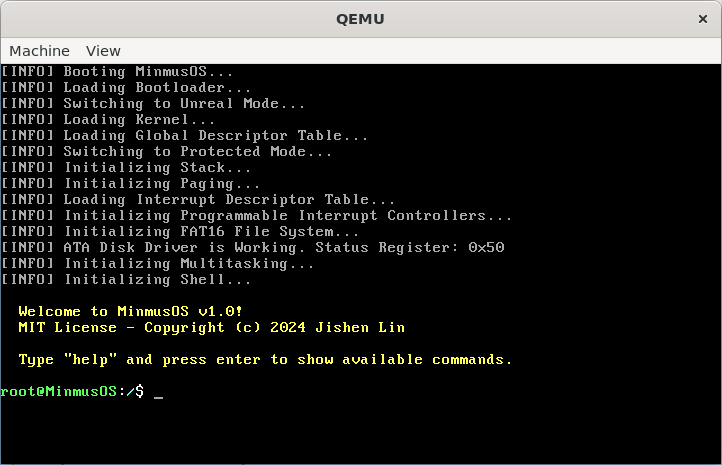
\includegraphics[width=0.8\textwidth]{figures/KernelBootPresentation.png}
    \caption{内核启动演示}
\end{figure}

\begin{figure}[htbp]
    \centering
    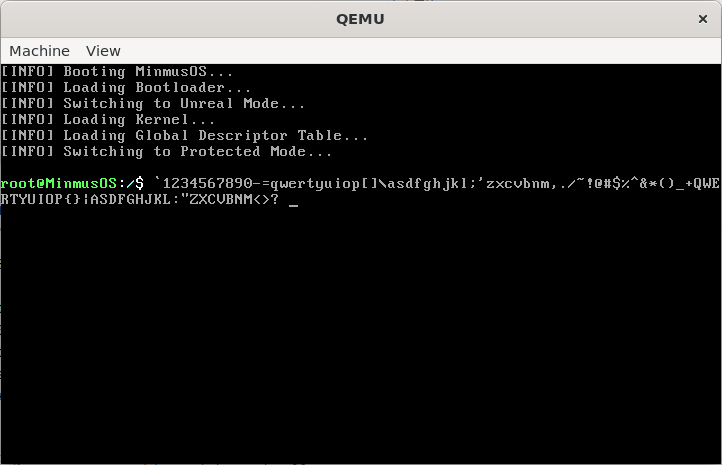
\includegraphics[width=0.8\textwidth]{figures/KeyboardDriverPresentation.png}
    \caption{键盘驱动程序演示}
\end{figure}

\begin{figure}[htbp]
    \centering
    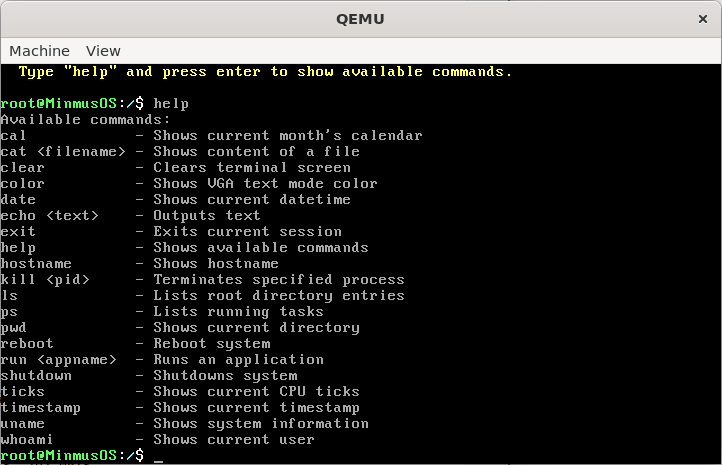
\includegraphics[width=0.8\textwidth]{figures/HelpCommandPresentation.png}
    \caption{help命令演示}
\end{figure}

\begin{figure}[htbp]
    \centering
    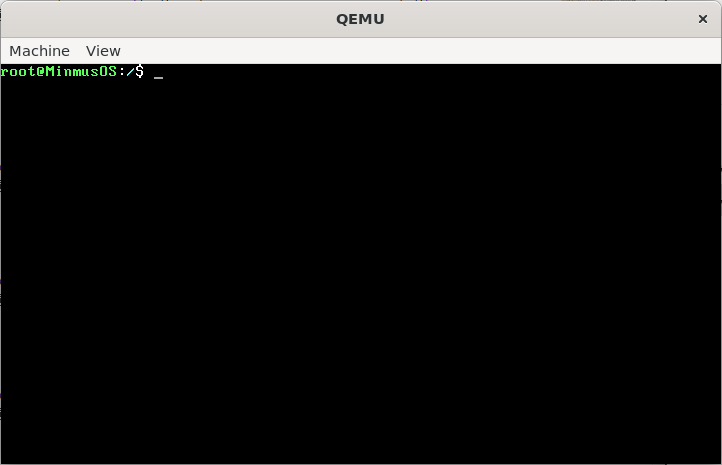
\includegraphics[width=0.8\textwidth]{figures/ClearCommandPresentation.png}
    \caption{clear命令演示}
\end{figure}

\begin{figure}[htbp]
    \centering
    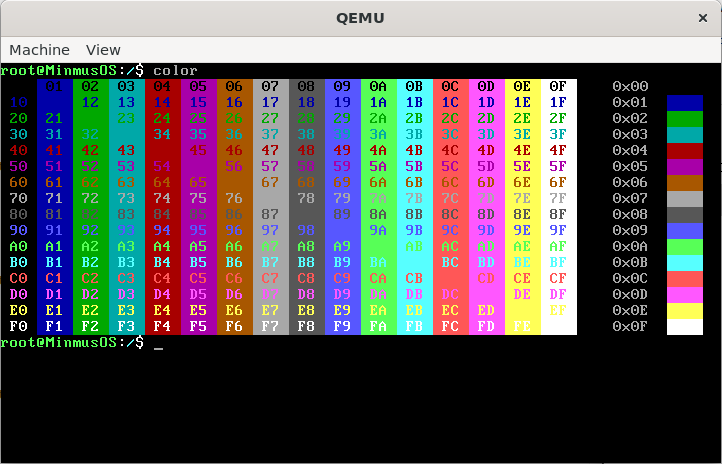
\includegraphics[width=0.8\textwidth]{figures/ColorCommandPresentation.png}
    \caption{color命令演示}
\end{figure}

\begin{figure}[htbp]
    \centering
    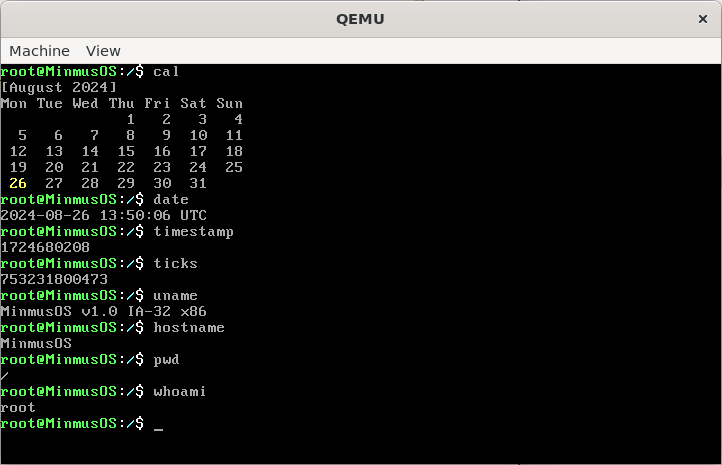
\includegraphics[width=0.8\textwidth]{figures/CalDateTimestampTicksUnameHostnamePwdWhoamiCommandPresentation.png}
    \caption{clear、date、timestamp、ticks、uname、hostname、pwd、whoami命令演示}
\end{figure}

\begin{figure}[htbp]
    \centering
    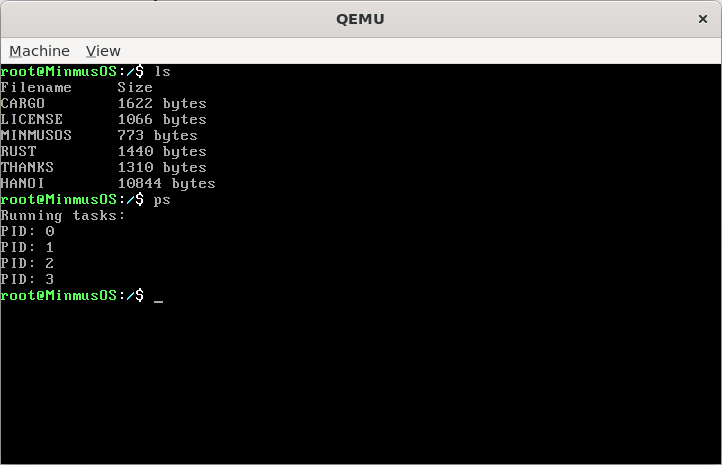
\includegraphics[width=0.8\textwidth]{figures/LsPsCommandPresentation.png}
    \caption{ls、ps命令演示}
\end{figure}

\begin{figure}[htbp]
    \centering
    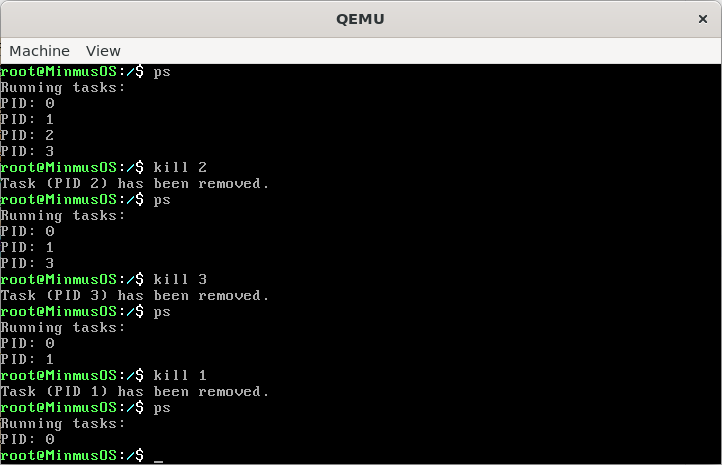
\includegraphics[width=0.8\textwidth]{figures/KillCommandPresentation.png}
    \caption{kill命令演示}
\end{figure}

\begin{figure}[htbp]
    \centering
    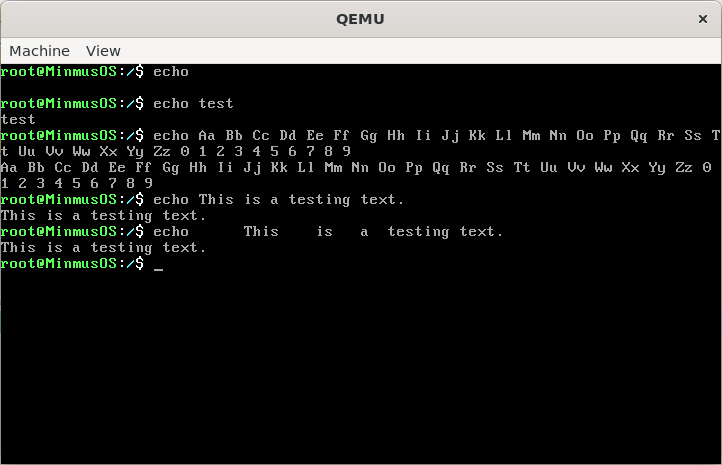
\includegraphics[width=0.8\textwidth]{figures/EchoCommandPresentation.png}
    \caption{echo命令演示}
\end{figure}

\begin{figure}[htbp]
    \centering
    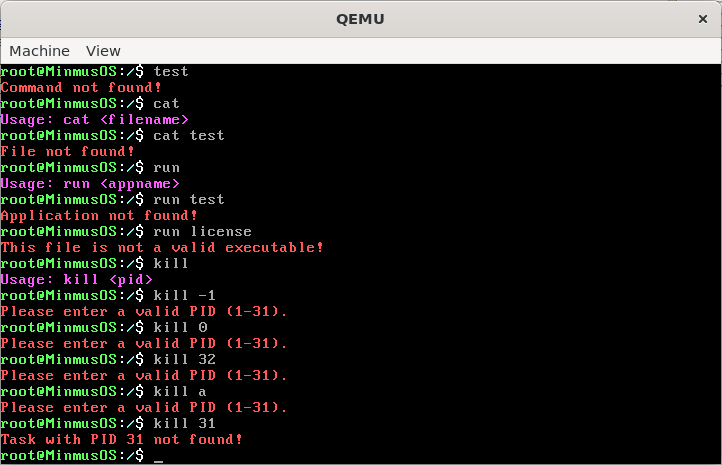
\includegraphics[width=0.8\textwidth]{figures/ErrorCommandPresentation.png}
    \caption{命令行解释器错误提示演示}
\end{figure}

\begin{figure}[htbp]
    \centering
    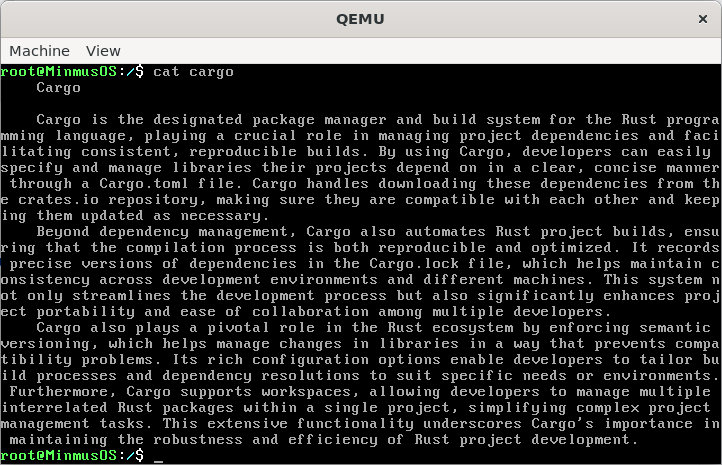
\includegraphics[width=0.8\textwidth]{figures/CargoFilePresentation.png}
    \caption{文本文件cargo演示}
\end{figure}

\begin{figure}[htbp]
    \centering
    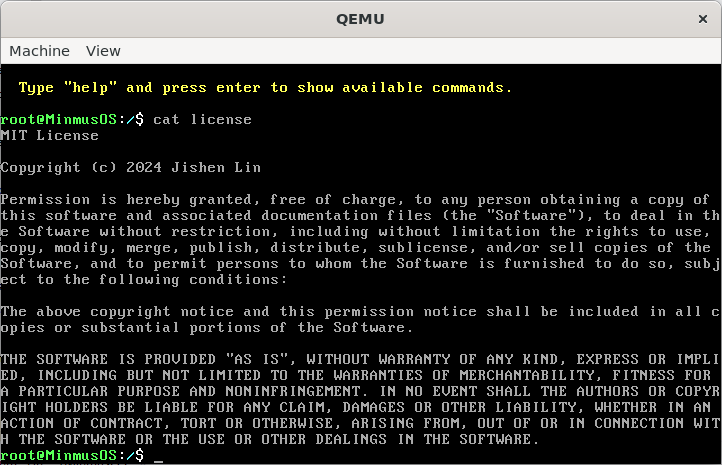
\includegraphics[width=0.8\textwidth]{figures/LicenseFilePresentation.png}
    \caption{文本文件license演示}
\end{figure}

\begin{figure}[htbp]
    \centering
    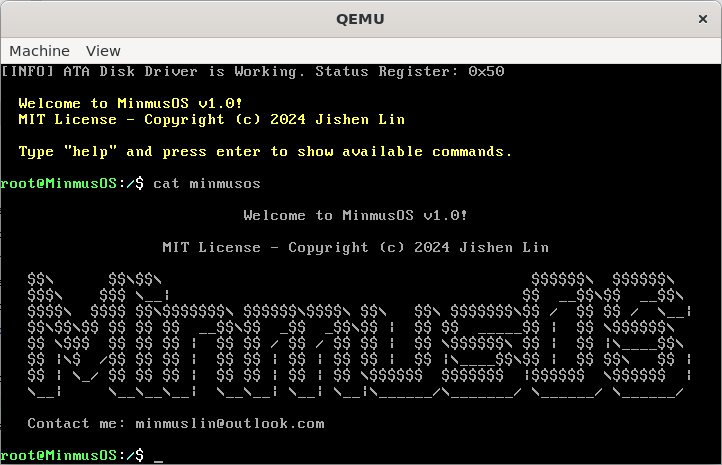
\includegraphics[width=0.8\textwidth]{figures/MinmusOSFilePresentation.png}
    \caption{文本文件minmusos演示}
\end{figure}

\begin{figure}[htbp]
    \centering
    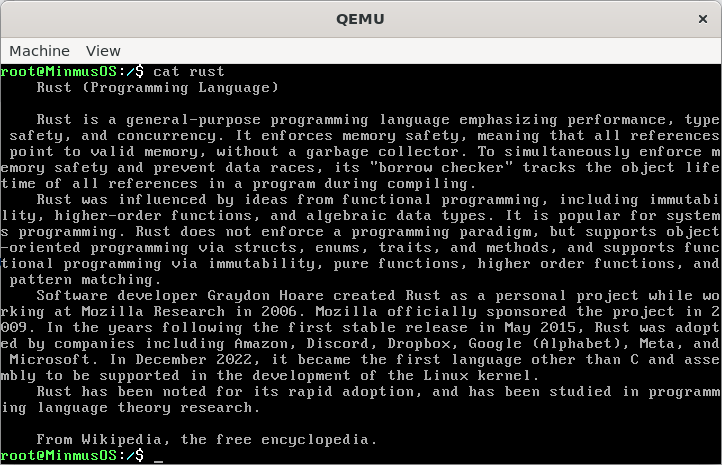
\includegraphics[width=0.8\textwidth]{figures/RustFilePresentation.png}
    \caption{文本文件rust演示}
\end{figure}

\begin{figure}[htbp]
    \centering
    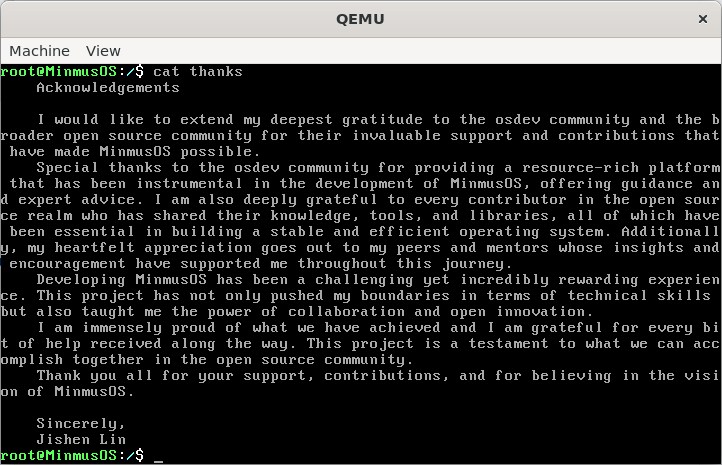
\includegraphics[width=0.8\textwidth]{figures/ThanksFilePresentation.png}
    \caption{文本文件thanks演示}
\end{figure}

\begin{figure}[htbp]
    \centering
    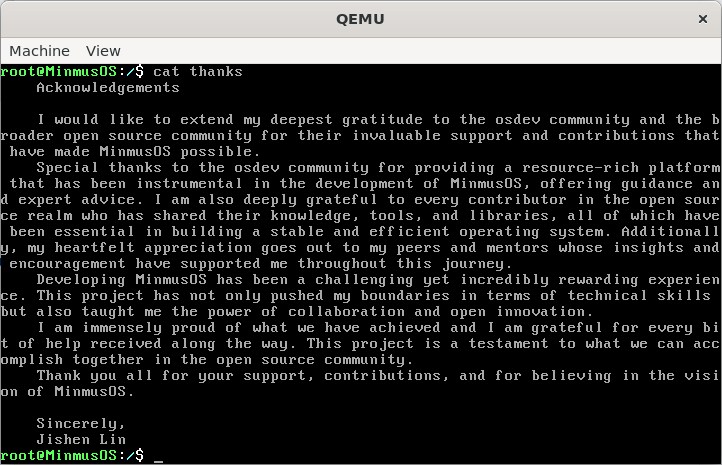
\includegraphics[width=0.8\textwidth]{figures/ThanksFilePresentation.png}
    \caption{文本文件thanks演示}
\end{figure}

\begin{figure}[htbp]
    \centering
    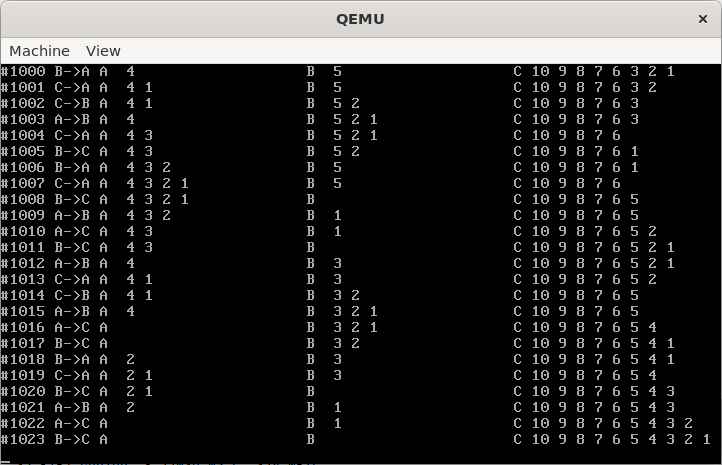
\includegraphics[width=0.8\textwidth]{figures/ApplicationHanoiPresentation.png}
    \caption{应用程序汉诺塔解决方案演示}
\end{figure}

\begin{figure}[htbp]
    \centering
    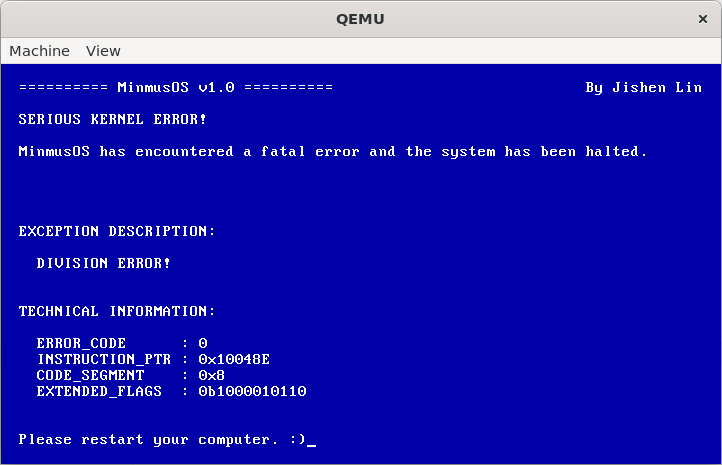
\includegraphics[width=0.8\textwidth]{figures/Exception0Presentation.png}
    \caption{0号异常演示:除零错误}
\end{figure}

\begin{figure}[htbp]
    \centering
    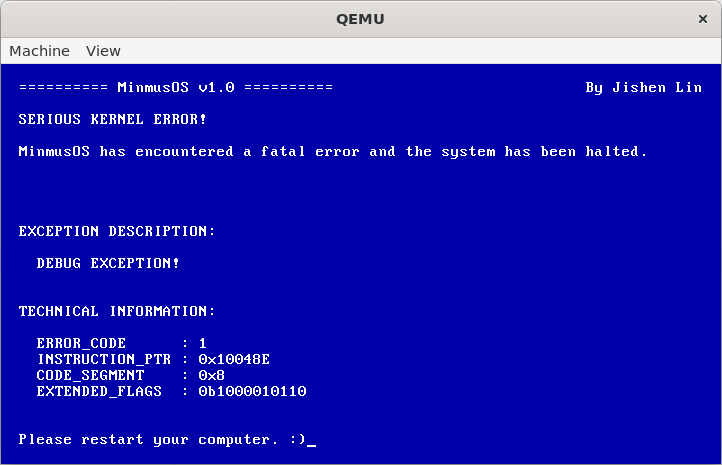
\includegraphics[width=0.8\textwidth]{figures/Exception1Presentation.png}
    \caption{1号异常演示:调试异常}
\end{figure}

\begin{figure}[htbp]
    \centering
    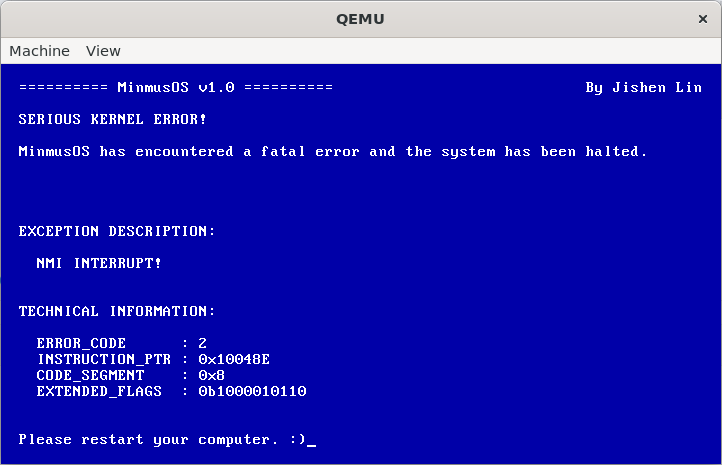
\includegraphics[width=0.8\textwidth]{figures/Exception2Presentation.png}
    \caption{2号异常演示:NMI中断}
\end{figure}

\begin{figure}[htbp]
    \centering
    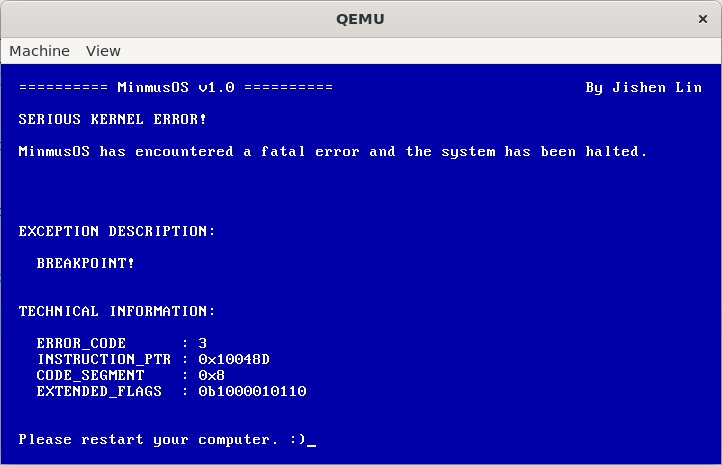
\includegraphics[width=0.8\textwidth]{figures/Exception3Presentation.png}
    \caption{3号异常演示:断点}
\end{figure}

\begin{figure}[htbp]
    \centering
    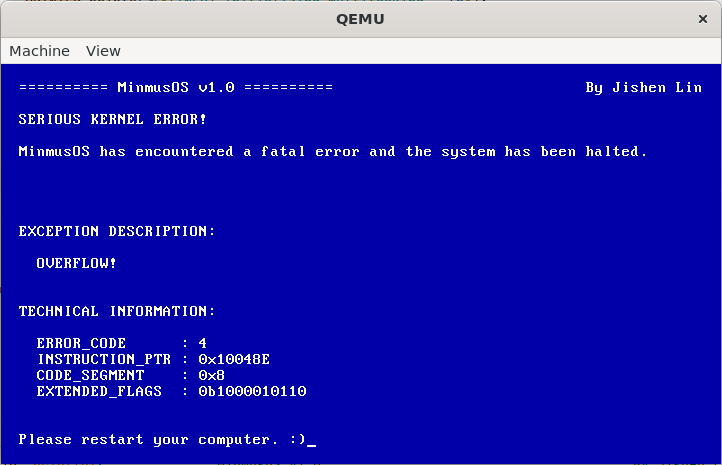
\includegraphics[width=0.8\textwidth]{figures/Exception4Presentation.png}
    \caption{4号异常演示:溢出}
\end{figure}

\begin{figure}[htbp]
    \centering
    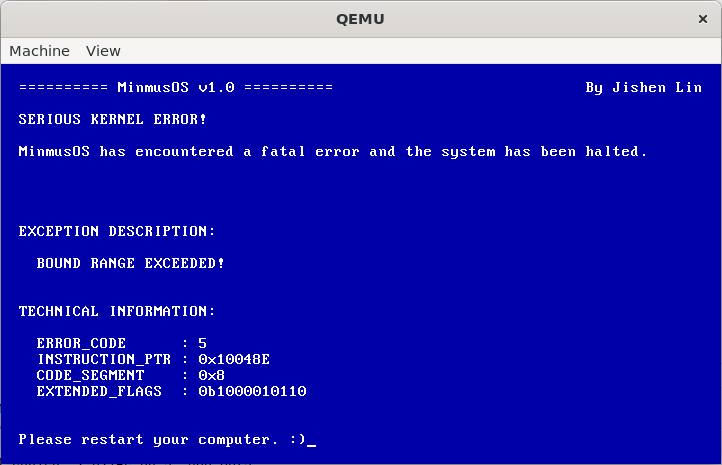
\includegraphics[width=0.8\textwidth]{figures/Exception5Presentation.png}
    \caption{5号异常演示:BOUND范围超出}
\end{figure}

\begin{figure}[htbp]
    \centering
    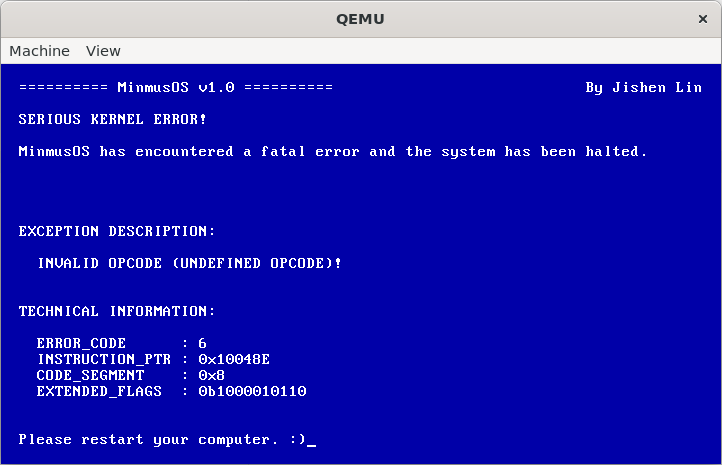
\includegraphics[width=0.8\textwidth]{figures/Exception6Presentation.png}
    \caption{6号异常演示:无效操作码(未定义操作码)}
\end{figure}

\begin{figure}[htbp]
    \centering
    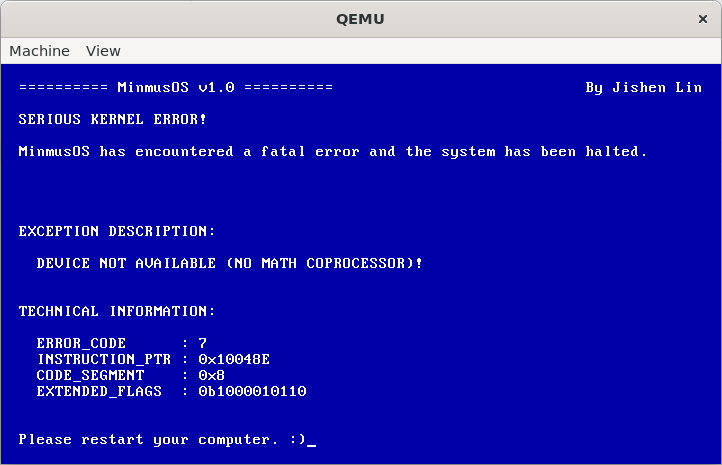
\includegraphics[width=0.8\textwidth]{figures/Exception7Presentation.png}
    \caption{7号异常演示:设备不可用(无数学协处理器)}
\end{figure}

\begin{figure}[htbp]
    \centering
    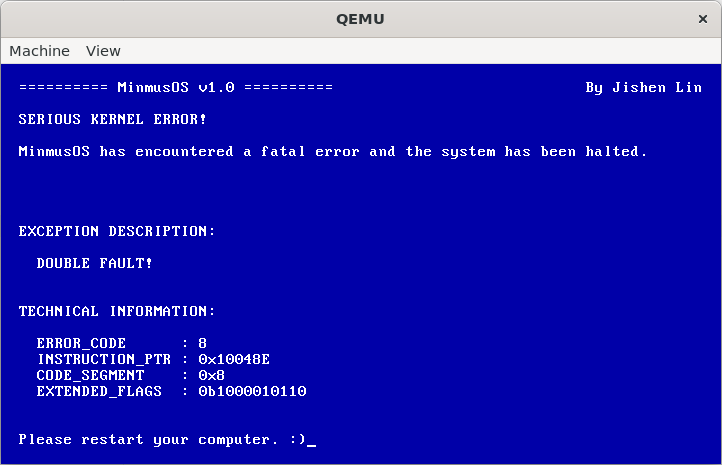
\includegraphics[width=0.8\textwidth]{figures/Exception8Presentation.png}
    \caption{8号异常演示:双重故障}
\end{figure}

\begin{figure}[htbp]
    \centering
    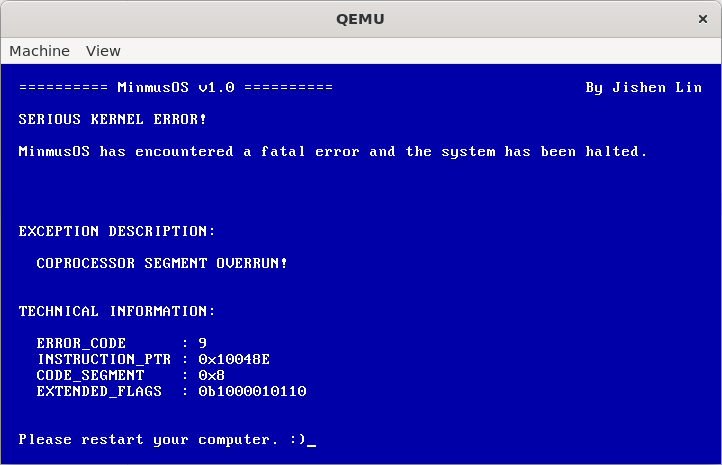
\includegraphics[width=0.8\textwidth]{figures/Exception9Presentation.png}
    \caption{9号异常演示:协处理器段溢出(保留)}
\end{figure}

\begin{figure}[htbp]
    \centering
    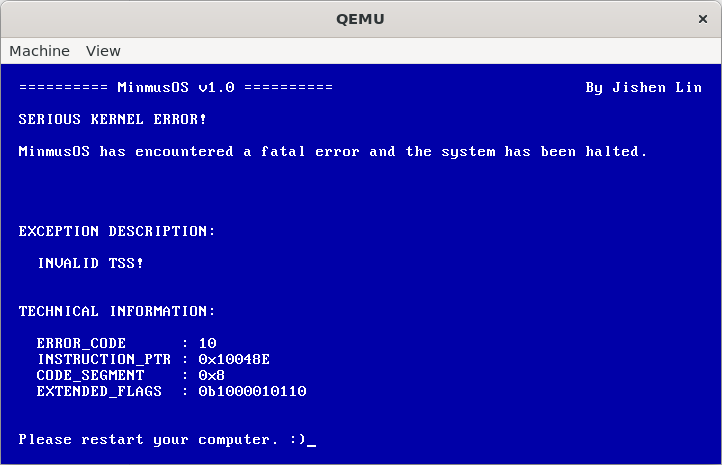
\includegraphics[width=0.8\textwidth]{figures/Exception10Presentation.png}
    \caption{10号异常演示:无效的TSS}
\end{figure}

\begin{figure}[htbp]
    \centering
    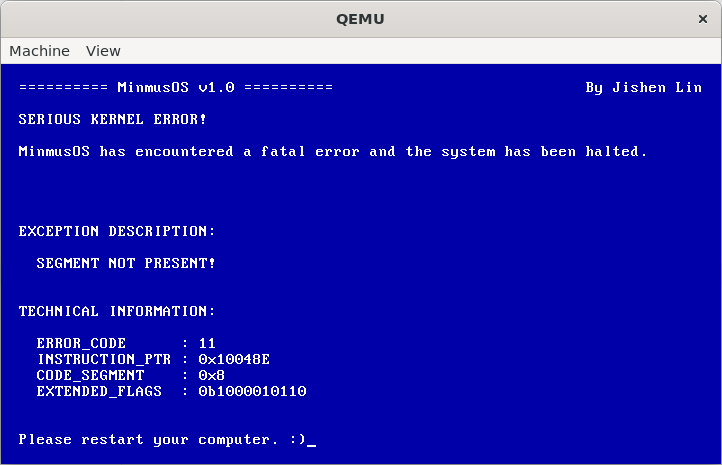
\includegraphics[width=0.8\textwidth]{figures/Exception11Presentation.png}
    \caption{11号异常演示:段不存在}
\end{figure}

\begin{figure}[htbp]
    \centering
    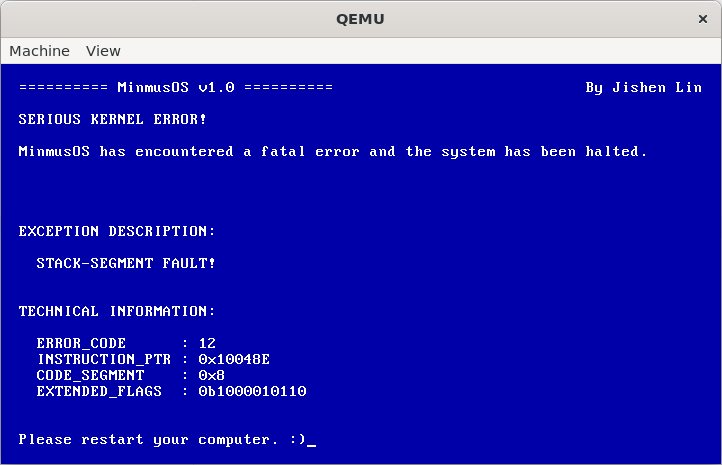
\includegraphics[width=0.8\textwidth]{figures/Exception12Presentation.png}
    \caption{12号异常演示:栈段故障}
\end{figure}

\begin{figure}[htbp]
    \centering
    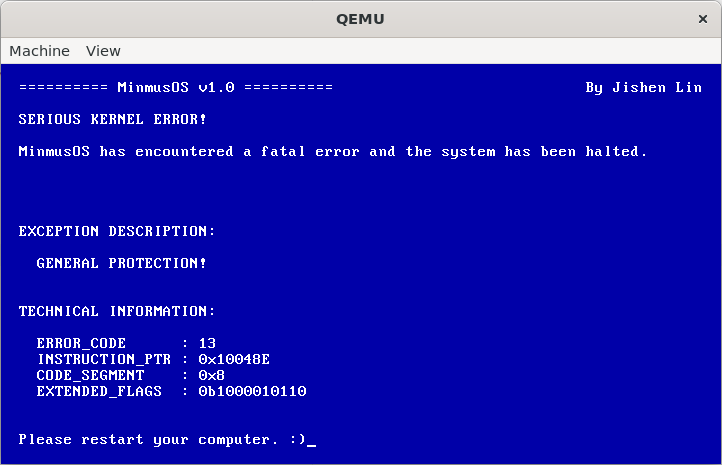
\includegraphics[width=0.8\textwidth]{figures/Exception13Presentation.png}
    \caption{13号异常演示:通用保护}
\end{figure}

\begin{figure}[htbp]
    \centering
    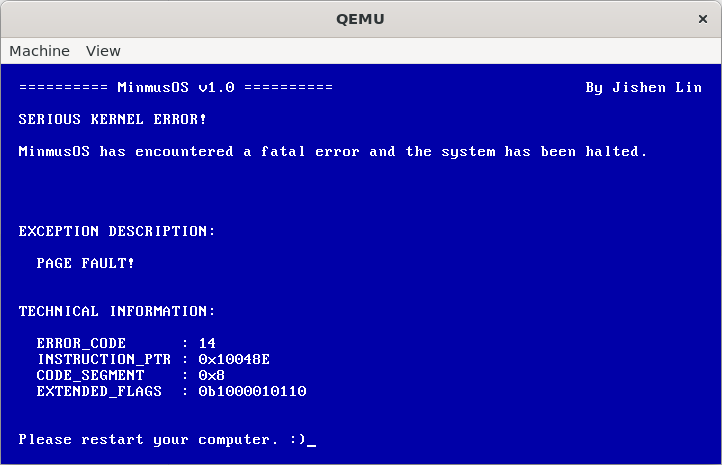
\includegraphics[width=0.8\textwidth]{figures/Exception14Presentation.png}
    \caption{14号异常演示:页面错误}
\end{figure}

\begin{figure}[htbp]
    \centering
    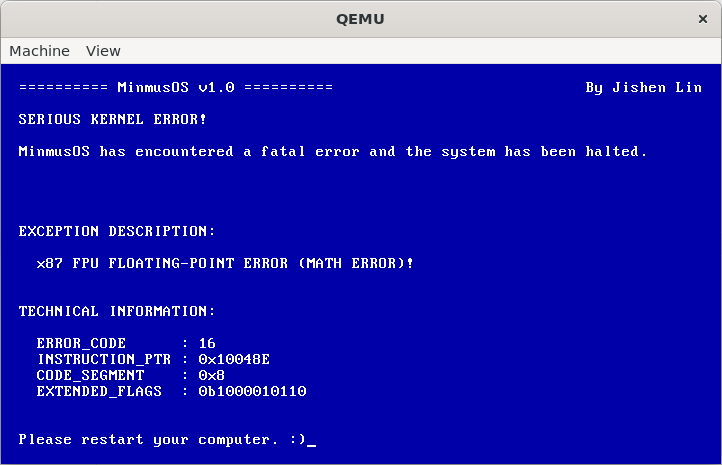
\includegraphics[width=0.8\textwidth]{figures/Exception16Presentation.png}
    \caption{16号异常演示:x87 FPU 浮点错误(数学故障)}
\end{figure}

\begin{figure}[htbp]
    \centering
    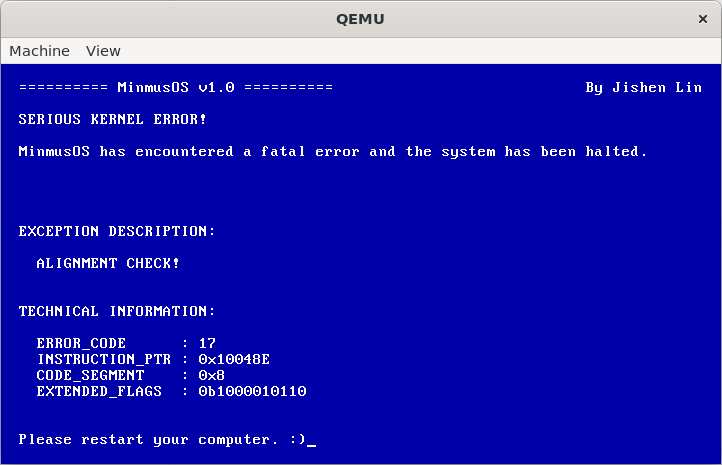
\includegraphics[width=0.8\textwidth]{figures/Exception17Presentation.png}
    \caption{17号异常演示:对其检查}
\end{figure}

\begin{figure}[htbp]
    \centering
    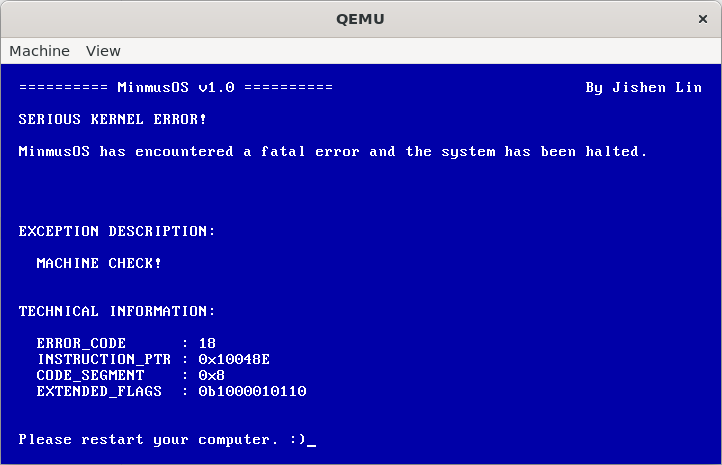
\includegraphics[width=0.8\textwidth]{figures/Exception18Presentation.png}
    \caption{18号异常演示:机器检查}
\end{figure}

\begin{figure}[htbp]
    \centering
    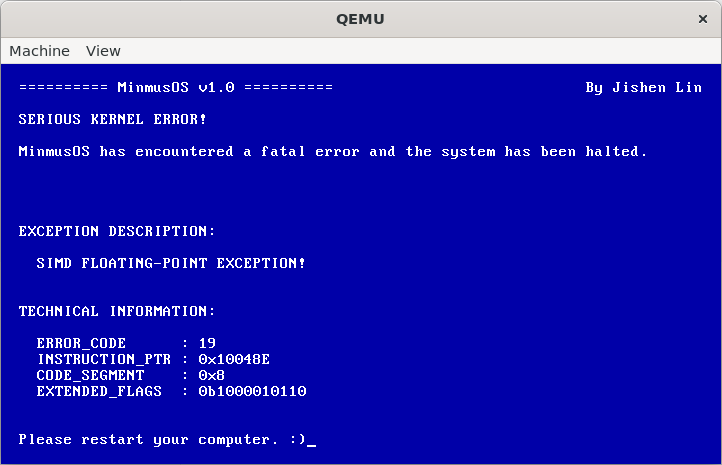
\includegraphics[width=0.8\textwidth]{figures/Exception19Presentation.png}
    \caption{19号异常演示:SIMD浮点异常}
\end{figure}

\begin{figure}[htbp]
    \centering
    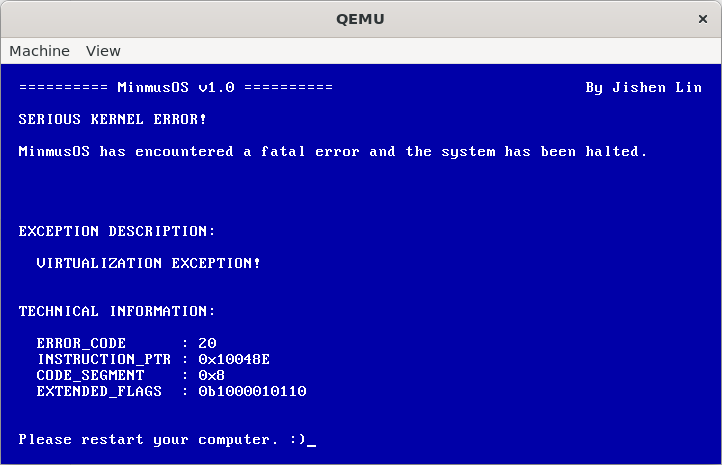
\includegraphics[width=0.8\textwidth]{figures/Exception20Presentation.png}
    \caption{20号异常演示:虚拟化异常}
\end{figure}

\begin{figure}[htbp]
    \centering
    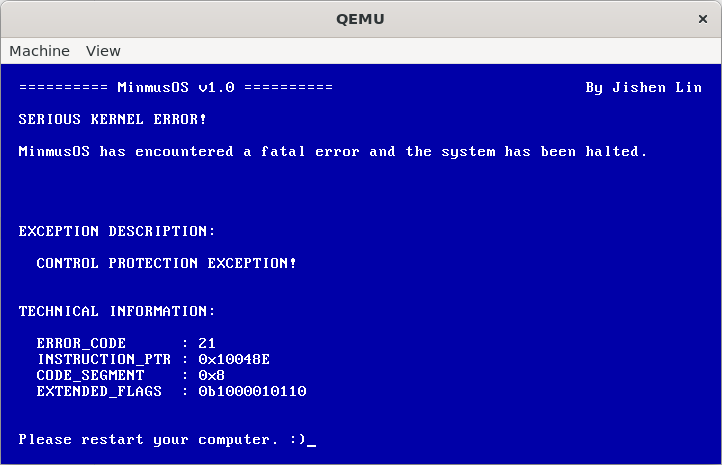
\includegraphics[width=0.8\textwidth]{figures/Exception21Presentation.png}
    \caption{21号异常演示:控制保护异常}
\end{figure}

\begin{figure}[htbp]
    \centering
    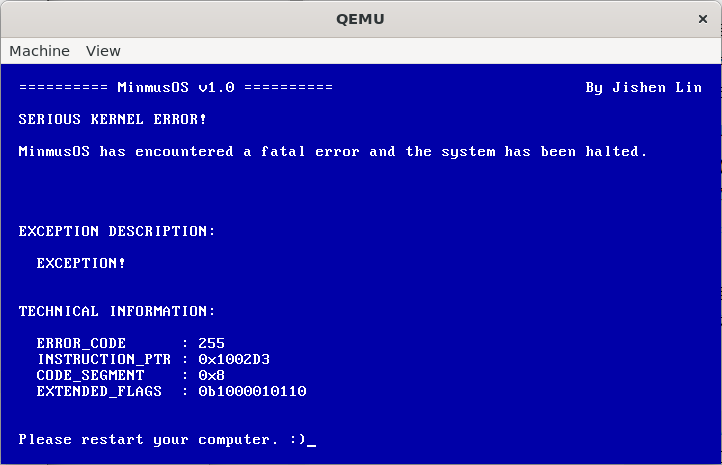
\includegraphics[width=0.8\textwidth]{figures/ExceptionHandlerPresentation.png}
    \caption{默认异常演示:Intel保留}
\end{figure}

\begin{figure}[htbp]
    \centering
    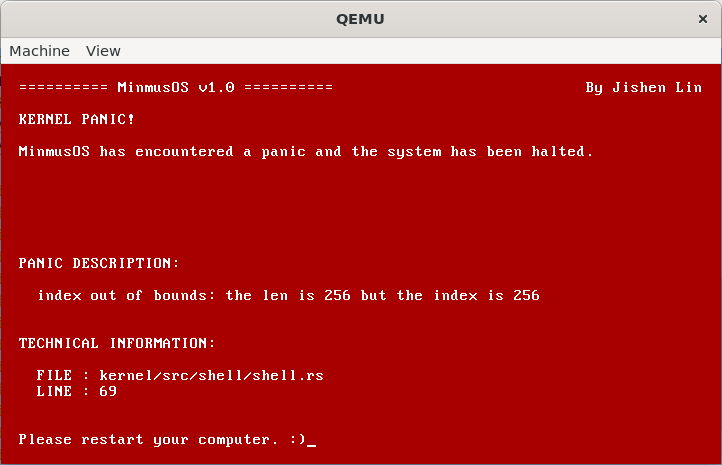
\includegraphics[width=0.8\textwidth]{figures/PanicHandlerPresentation.png}
    \caption{PANIC演示:索引越界}
\end{figure}

\begin{figure}[htbp]
    \centering
    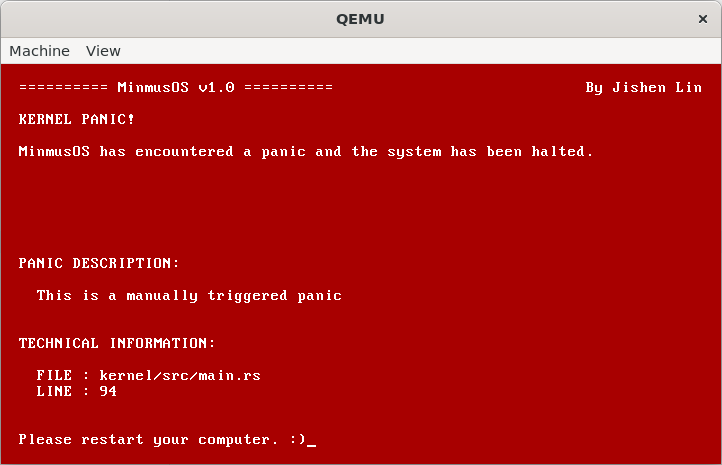
\includegraphics[width=0.8\textwidth]{figures/ManuallyTriggeredPanicPresentation.png}
    \caption{PANIC演示:手动触发PANIC}
\end{figure}